%\documentclass[12pt]{apa7}
\documentclass[man, noextraspace, floatsintext, 12pt]{apa7}
%\documentclass[12pt, noextraspace, floatsintext]{apa6}
%\documentclass[man, 12pt, noextraspace, floatsintext]{apa6}
%\documentclass[11pt]{article}

% ADD REVIEWING PACKAGE
\usepackage{easyReview}
% Show reviews/edits or not?
\setreviewson
%\setreviewsoff
% Line numbers for ease of pointing to lines
\usepackage{lineno} %[pagewise]
%\linenumbers

\usepackage{lscape}
%Math typesetting packages
\usepackage{amsfonts, amssymb, amsmath, latexsym, amsthm}
%for URLs in-text 
\usepackage{url}
% ================
% = Bibliography =
% ================
%APA style citations and references
%\usepackage[utf8]{inputenc}
%\usepackage{babel,csquotes,xpatch}
\usepackage[backend=biber, style=apa, natbib, sortcites]{biblatex}
\addbibresource{references.bib}

%\usepackage[natbibapa]{apacite} 
% for hanging-indentation style using apacite
%\setlength{\bibindent}{2.5em}
%\setlength{\bibleftmargin}{0em}
% ==========
% = Floats =
% ==========
\usepackage{float}
% include external pictures
\usepackage{graphicx} %Graphics/figures
% rotate figures/tables
\usepackage{rotating} 
% For professional tables
\usepackage{booktabs,threeparttable, multirow} 
\usepackage{tabularx}
% For fixing the column widths
\usepackage{array}
\newcolumntype{L}[1]{>{\raggedright\let\newline\\\arraybackslash\hspace{0pt}}m{#1}}
\newcolumntype{C}[1]{>{\centering\let\newline\\\arraybackslash\hspace{0pt}}m{#1}}
\newcolumntype{R}[1]{>{\raggedleft\let\newline\\\arraybackslash\hspace{0pt}}m{#1}}

% ===================
% ==== Tikz Diagrams	==
% ===================
\usepackage{tikz}
\usetikzlibrary{calc,arrows,positioning,shapes,shapes.gates.logic.US,trees, intersections}
% =======================
% === Other useful packages ==
% =======================
\usepackage[T1]{fontenc} 
\usepackage{placeins}
\usepackage{hyperref}
% subcaptions/subfigures %,justification=centered
\usepackage[hypcap=true,width=\textwidth]{subcaption}
% =============
%  == formatting ==
% =============
% \usepackage[margin=1in]{geometry}
% \setlength{\parindent}{0.5in}
\usepackage{setspace}
% \doublespacing

% ==========
% = Syntax =
% ==========
% For Computer Code in Appendix. I set the language for R, so will need to be changed for different languages
\usepackage{listings}
\lstset{
    language=R,
    basicstyle=\small \ttfamily,
    commentstyle=\ttfamily ,
    showspaces=false,
    showstringspaces=false,
    showtabs=false,
    frame=none,
    tabsize=2,
    captionpos=b,
    breaklines=true,
    breakatwhitespace=false,
    title=\lstname,
    aboveskip=10pt,
    belowskip=-10pt,
    %escapeinside={},
    %keywordstyle={},
    %morekeywords={}
    }%
%~~
\title{Assessing local fit by approximating probabilities}
\shorttitle{Assessing local fit} % For APA package
\author{R. Noah Padgett}
%\author{Graduate Student}
\authorsaffiliations{Baylor University}
%\affiliation{REMOVED FOR PEER REVIEW}



\abstract{Validity evidence for factor structures underlying a set of items can be based on how well a proposed model reconstructs, or fits, the relationships among observed variables. Global model fit is limited in that some components of the proposed model fit better than other components. This limitation has led to the recommendation of examining fit locally within model components. In this study, we describe a new probabilistic approach to assessing local fit using a Bayesian approximation, and illustrate the use of the proposed approach to assessing local fit with a simulated dataset. We also show how the posterior approximation closely approximated the sampling distribution of the true parameter. Finally, we discuss potential limitations and possible generalizations.
%\singlespacing
 } % End abstract

\keywords{local fit, factor analysis, Laplace, posterior probability}

%\authornote{REMOVED FOR PEER REVIEW}
\authornote{
R. Noah Padgett, Department of Educational Psychology, Baylor University.

Correspondence concerning this article should be address to R. Noah Padgett, Department of Educational Psychology, One Bear Place \# 97304, Baylor University, Waco, TX 76798. Contact: \href{mailto:noah\_padgett1@baylor.edu}{\tt noah\_padgett1@baylor.edu}
}


\begin{document}

\maketitle

%% Spacing for Eqations Can't be in preamble...
\setlength{\abovedisplayskip}{3pt}
\setlength{\belowdisplayskip}{3pt}

Statistical models, such as structural equation models, are intended to serve as an approximation of the process or mechanisms through which data generated.
The approximation of reality has been described as arising from distributional and structural approximations \citep{Bollen2019}.
When models fail to closely approximate reality (i.e., misfit), identifying the source(s) of model misspecifications can be at best, difficult, and at worst, impossible.
Fortunately, a variety of methods are available to aid researchers in evaluating the fit of their proposed model for measuring one or more constructs \citep{DiStefano2016}. 
In fact, statistical information that demonstrates acceptable model-data fit can be taken as evidence for a measurement models construct validity.

One popular method of collecting evidence supporting one's proposed model involves the use of global fit indices.
Global fit indices help identify whether the specified measurement model adequately approximates the data generating process overall. 
Commonly used global fit indices are the comparative fit index \citep{Bentler1990},  root mean square error of approximation \citep{Browne1992}, and standardized root mean square residual \citep{Bentler1995, Maydeu2018, Joreskog1981}.
Many of these indices are now automatically computed in most SEM software.
However, these indices only provide a coarse estimate of overall model-data fit \citep{Steiger2007}.

One difficulty arising from the coarse nature of global fit indices is that when the indices are below acceptable values a researcher must explain the lack of fit. 
Global fit indices do not necessarily help identify where the misspecification is occurring though.
Some parts of the model may better represent the latent structure than other parts, but identifying which parts are not representative is not straightforward.
Methods of identifying the source of misfit include investigating residual matrices \citep{Kline2015, Maydeu2017}, modification indices \citep{Sorbom1989, Kaplan1989}, Wald tests \citep{Wald1943, Buse1982}, likelihood ratio tests \citep{Neyman1928, Buse1982}, and model-implied instrumental variables \citep{Bollen1995, Bollen2019}.
Each method has benefits and pitfalls that need to be considered when looking for evidence of model-data fit. 
The methods above generally provide users with a way of identifying which specific relationships among observed variables are not captured by the model (e.g., residuals) or which specific component of the model does not fit well (e.g., Wald tests).
Once a change in the model has been made, a researcher can then compare the results of local fit to see if fit improved.

Evaluating the change in model fit has been helpful for many in the model fit evaluation process as evident by the prolonged use of these approaches, but this process has potential drawbacks.
For example, modification indices can produce conflicting information about sources of misfit, which can in turn lead to statistically equivalent models.
Adding too many paths to the measurement or structural components of the model may result in and difficulty interpreting model parameters due to model overfit.
Aside from investigating standardized residuals \citep{Maydeu2017}, most current methods of investigating local fit rely on non-intuitive metrics, such as modification indices, likelihood ratios, or p-values.
In order to improve the interpretability of local fit investigations, we propose an approach utilizing probabilities as the inferential unit for local fit assessment. 
In the proposed probabilistic approach, the aim is to approximate whether additional paths will result in a meaningfully interpretable contribution to the model.
Our method helps control against overfit through interpretation-driven local fit assessment.

There are numerous important contributions of this work.
First, we extend previous research on local fit assessment by introducing a probabilistic method utilizing Bayesian methods. 
Second, we demonstrate the application of this approach in a simulated dataset with a known latent structure.
Finally, we investigated the performance through Monte Carlo simulation study evaluating the accuracy of the predicted probabilities.

\subsection{Proposed probabilistic method for local fit assessment}

Local fit assessment by means of investigating residual matrices, modification indices, Wald tests, likelihood ratio tests or model-implied instrumental variables have each shown to provide useful information in a variety of contexts \citep{Chou1990, Whittaker2012, Maydeu2017}.
However, these methods fail to reflect whether potential model modifications would result in a change in substantive interpretation of the model.  
To address this issue, we have developed a relatively straightforward approach to evaluate local fit by means of an iterative approximation of the non-estimated parameters.

The proposed method approximates the magnitude of the non-estimated parameters if added to the model, where magnitude is approximated by a probability distribution to represent the uncertainty in the parameter. 
Using the distribution of each parameter, a probability can be computed to capture how likely that the parameter would be of substantive interest.
The idea underlying this approach to local fit assessment is to define a region of the parameter space that would be considered meaningful for the substantive question at hand. 
A natural choice in the case of factor loadings is to define the region as $\vert \lambda \vert \geq 0.30$ \citep{Benson1998}, which is the threshold typically considered as the bound for standardized factor loadings in exploratory factor analysis (EFA).
However, we are not restricted to this region; for example, we might be interested in knowing if any loadings would likely be greater than one, indicating that the item loads more strongly than the item we fixed for identification.
This approach is similar to defining a ``region of practical equivalence (ROPE)'' described in \textcite{Shi2019} as a Bayesian approach for measurement invariance testing.
The ROPE is a region in the parameter space that the researcher determines to be insignificant, which is already common in most applications of EFA when the researcher suppresses factor loadings that are below 0.30 \citep{Benson1998}.

The proposed to local fit assessment defines regions of the parameter space that are of practical insignificance and then approximates the probability that our model parameters fall in that space.
The probabilities are based on a rough approximation of a posterior distribution based on Bayes theorem.
A similar quantity in Bayesian methods is the posterior predictive probability \citep[PPP or $p$-value, ][]{Gelman1996, Rubin1996}.
The PPP is often used to construct probabilistic inferences about test statistics from the posterior predictive distribution.
However, for the current application we are interested in computing a probability based on the posterior itself leading to a simpler approximation problem.
 
\textcite{Lee2016} discussed a related approach whereby posterior approximation helps evaluate global model fit and identify influential observations.
The authors suggested that the probabilistic approach can be used to assess model fit in a variety of ways such as residual covariances.
Yet no one yet has built on this method for investigations of local fit assessment, and therefore, it is the focus of our work.
Next, we briefly review the necessary aspects of Bayesian theory needed for the probability of inferential interest.

\subsubsection{Bayesian methods underlying the assessment of local fit}

Bayes theorem is one of the most powerful tools to manipulate probabilities. 
Bayes theorem provides a framework for decomposing a conditional probability into a likelihood statement about observed data and a hypothesized probability space for model parameters (i.e., the prior).
This can be expressed:
\begin{align*}
p(\theta \vert Y) \propto \ell (Y \vert \theta)p(\theta),
\end{align*}
where $\propto$ is read as ``proportional to'', $\ell (Y \vert \theta)$ is the likelihood of the data $Y$ determined by the model specified and parameters $\theta$, and $p(\theta)$ is the joint prior distribution for the parameters in the model.
The posterior is usually sampled from using Monte Carlo methods (e.g., Gibbs sampling, Hamiltonian Monte Carlo, etc.).
However, in this case we elect to utilize a \textit{relatively} simpler approximation of the posterior from which we can sample from relatively quickly.

Under mild regularity conditions of smoothness of the likelihood function, the posterior distribution for $\theta$ will approximate a normal distribution as the number of samples drawn from the distribution increases \citep{DBA3}.
Using this property of the posterior, Laplace's method can be used to derive a second-order Taylor series approximation to the posterior \citep{Tierney1986}.
The Taylor series approximation provides a point estimate for the posterior expectation and variance.
Then, using these two pieces matched with the knowledge that the posterior is asymptotically normally distributed, we arrive at an approximate posterior distribution for any parameter. 
The Laplace approximation has been shown to provide a useful approximation of posteriors for relatively simple models in a variety of contexts \citep{Kass1989, Rue2009}.

Under the same regularity conditions that allow us to assume the normal distribution we would get that that $\hat{\theta}$ under the Laplace approximation is nearly equal to $\hat{\theta}_{MLE}$ and that the variance under the Laplace approximation is nearly identical to the $I_{OBS}$  (the observed information). %$\hat{\theta} \approx \hat{\theta}_{MLE}$ and that $-\ddot{q}(\hat{\theta}) \approx I_{OBS}$ (the observed information).
Excluding the prior distribution for $\theta$ in the approximation has been used previously \citep{Lee2016, Rue2009, Wolfinger1993, Li1992}; however, excluding the prior decreases the uncertainty in the posterior distribution for $\theta$ even if only slightly.
Additionally, utilizing a minimally informative prior structure provides a useful initializing point for numerical methods.
Next, we will describe how Laplace's method can be applied in factor analysis for local fit assessment.

\subsubsection{Applying the Laplace approximation to Bayesian CFA}

Using the Bayesian factor analysis notation from\textcite{Levy2013}, the full model is
\begin{align} \label{eq:cfa}
\mathbf{Y}_i &= \tau + \Lambda \eta_i + \theta_i\\
\Sigma &= \Lambda^T \Phi \Lambda + \Theta \nonumber\\
\mathbf{Y}_i &\mid \tau, \Lambda, \eta_i, \Theta \sim \mathrm{N}\left(\tau + \Lambda \eta_i, \Theta \right) \nonumber \\
\eta_i &\mid \kappa, \Phi \sim \mathrm{N}\left(\kappa, \Phi \right) \nonumber
\end{align}
where $\mathbf{Y}_i$ is the response vector for person $i$, $\tau$ is the vector of indicator intercepts, $\Lambda$ is the matrix of factor loadings, $\eta_i$ is the vector of factor scores, $\theta_i$ is the vector of residuals, $\Sigma$ is the indicator/observed variable covariance matrix, $\Theta$ is the error covariance matrix, $\kappa$ is the vector of factor intercepts (usually fixed to 0), and $\Phi$ is the factor covariance matrix.
The full model could be incorporated in a Bayesian perspective relatively easily, but the parameter space grows rapidly.
Below is one potential way the full joint posterior could be express.
\begin{equation} \label{eg:post}
\pi\left(\tau, \Lambda, \eta,\Theta, \kappa, \Phi\mid \mathrm{Y}\right) \propto \ell\left(\mathrm{Y} \mid \tau, \Lambda, \eta,\Theta, \kappa, \Phi\right) \times \pi\left(\tau, \Lambda, \eta,\Theta, \kappa, \Phi\right),
\end{equation}
which increases in complexity as the large number of subjects, items, and latent variables increases.
The likelihood is not difficult to define due to the assumption of conditional independence of subjects, and further simplification can be made if conditional independence of items is assumed (i.e., $\Theta$ is a diagonal matrix)
\begin{align*}
\ell\left(\mathrm{Y} \mid \tau, \Lambda, \eta,\Theta, \kappa, \Phi\right) &= \prod_{i=1}^{N} f\left(\mathbf{Y}_i \mid \tau, \Lambda, \eta_i, \Theta \right)\\
 &=\prod_{i=1}^{N} \prod_{j=1}^{J}f\left(Y_{ij} \mid \tau_j, \lambda_{j}, \eta_i, \theta_{jj} \right).
\end{align*}

A more complicated issue is on the construction of the joint prior distribution because constructing joint prior distributions directly in multiparameter problems is typically not possible outside of special cases (e.g, normal-gamma conjugate prior in normal theory multiple linear regression).
In multiparameter problems, a common method for building the joint prior distribution is to construct the prior hierarchically.
The hierarchical prior for factor models can be constructed by decomposing the prior into parameter groups that can defensibly be independent or at least conditionally independent.
A potential decomposition is to have independent groups for factor loadings ($\Lambda$), item intercepts ($\tau$), and error (co)variances ($\Theta$), then group the factor scores ($\eta$), factor intercepts ($\kappa$), and factor covariance matrix ($\Phi$) together.
The later grouping can be structured where the factor scores distribution is conditional on the factor intercept and factor covariance matrix priors.
Therefore, the decomposed prior could be expressed as
\begin{align*}
\pi\left(\tau, \Lambda, \eta,\Theta, \kappa, \Phi\right) &= \pi\left(\eta, \kappa, \Phi\right)\pi\left(\tau\right)\pi\left(\Lambda\right) \pi\left(\Theta\right)\\
&= \pi\left(\eta\mid \kappa, \Phi\right) \pi\left(\kappa\right)  \pi\left(\Phi\right) \pi\left(\tau\right)\pi\left(\Lambda\right) \pi\left(\Theta\right).
\end{align*}
Some common specifications of the priors for these parameters are
\begin{align*}
\eta\mid \kappa, \Phi &\sim \mathrm{N}(\kappa,\Phi)\\
\kappa &\sim \mathrm{N}(\mu_{\kappa}, \sigma^2_{\kappa})\\
\Phi &\sim \mathrm{Inverse-Wishart}(d\Phi_0, d),\ d \geq M\\
\tau_{j} &\sim \mathrm{N}(\mu_{\tau}, \sigma^2_{\tau})\\
\lambda_{jm} &\sim \mathrm{N}(\mu_{\lambda}, \sigma^2_{\lambda})\\
\theta_{jj} &\sim \mathrm{Inverse-Gamma}(\alpha_{\theta}, \beta_{\theta})\\
\theta_{jk} &\sim \mathrm{N}(\mu_{\theta}, \sigma^2_{\theta}).
\end{align*}
The indices $j$ correspond to the $j^{th}$ indicator and $m$ is index over latent variables.
The factor loadings, intercepts, error (co)variances may be specified independently for each individual parameter which greatly simplifies the process, but is not necessary.
If the error (co)variance matrix was not hypothesized to be diagonal, then that structure could be included as part of a joint prior on $\Theta$.

Once the joint prior is constructed, it may be difficult in a full Bayesian analysis to sample from the posterior.
A common solution is to employ some type of Markov Chain Monte Carlo (MCMC) algorithm to efficiently sample from the marginal posteriors of each parameter.
Several software options that make this job easier including blavaan \citep{blavaan}, JAGS \citep{jags}, M\textit{plus} \citep{Mplus}, OpenBUGS \citep{bugs}, and Stan \citep{Stan}.
That said, we propose a drastic simplification of the full Bayesian analysis with the aim of obtaining a rough approximation of a specific feature of the posterior.

As we have described previously, our aim is to \textit{approximate} the probability that a parameter is outside a region of practical importance (or that the absolute value exceeds a threshold).
MCMC methods can certainly be used for this purpose but our intent is to provide a simpler, quicker, and less computationally intensive approach that can be utilized as part of the model evaluation process for local fit assessment.
The complex posterior distribution is simplified as we shift from sampling from the marginal posterior to a specific conditional posterior for each parameter.
That is, observations are sampled from each posterior by fixing estimates of loadings, error (co)variances, factor (co)variances, etc. in order to reduce the model down to a single parameter problem.
Then, Laplace's method is employed to form a normal distribution approximation to the conditional posterior of parameter(s) of interest which we can then draw samples to from the approximated posterior.
The steps of the proposed algorithm are described in Appendix \ref{app:algorithm} and the code used for this algorithm is shown in Appendix \ref{app:code}.


\section{Illustrative Example of Local Fit Assessment with Simulated Data}

To illustrate the proposed method, consider the ``true'' factor model shown in Figure \ref{fig:model}.
The simple three factor structure was selected for illustrative purposes. 
Using a sample of 500 drawn from this model, a similar, yet misspecified model ignoring the residual covariances was estimated using \textsf{lavaan} \citep{Rosseel2012}.
\begin{figure}
\centering
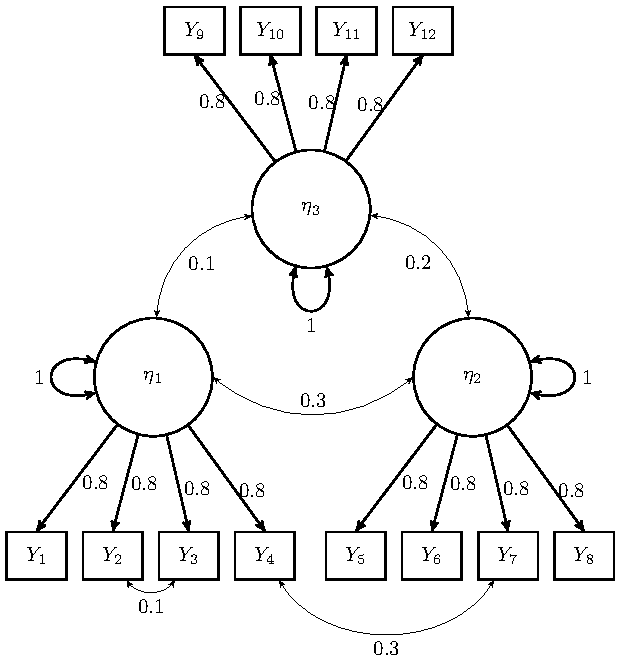
\includegraphics[width=0.5\textwidth]{fig/sim_factor_structure_values}
\caption{Simulating data model}
\label{fig:model}
\end{figure}
Based on the model $\chi^2$, the model does not fit these data $(\chi^2(51) = 124.3, p < 0.001)$.
Next,one must attempt to diagnose the source of inadequate model-data fit, such as which paths were not specified.
Next, we applied the described probabilistic approach to try to identify omitted paths that may be of substantive interest. 
The results from the proposed local fit assessment are shown in Table \ref{tb:prob}. 
The paths (i.e., loading or  error covariances) identified as most likely of substantive interest are shown in descending order.
For simplicity we are only showing the paths with the highest nine probabilities plus the covariance for $Y_2$ and $Y_3$.
These estimates are shown in Table \ref{tb:prob}.
We found that, with the method described in this paper, the path for the covariance between $Y_4$ and $Y_7$ had the highest probability of being meaningful in magnitude whereas the covariance between $Y_2$ and $Y_3$ was unlikely to be meaning.
This matches well with the true model where the covariance between $Y_4$ and $Y_7$ was 0.30 which is above the cutoff of 0.25 whereas the covariance between $Y_2$ and $Y_3$ was 0.10 in the population which is below the cutoff.


\begin{table}[ht]
\centering
\begin{threeparttable}
\caption{Estimated probabilities of parameters being outside region of practical equivalence}
\label{tb:prob}
\begin{tabular}{lr}
  \toprule
$\theta$ & $\mathrm{Pr}( \mid \theta \mid \geq {\rm cutoff})$\\ 
  \midrule
  	$\sigma_{7, 4}$ & \textbf{.998}\\ 
	$\lambda_{7, 1}$ &	.014\\
	$\sigma_{5,1}$ &	.012\\
	$\sigma_{11, 4}$ &	.009\\
	$\lambda_{6, 1}$ &	.005\\
	$\sigma_{9, 7}$ &	.004\\
	$\sigma_{3, 2}$ &	\textbf{.001}\\   \bottomrule
\end{tabular}
\vspace*{1mm}
 	\begin{tablenotes}[para,flushleft]
    {\small
        \textit{Note.} Bolded values are for parameters that are from the true generating model. Cutoff for $\sigma$ was 0.25 and cutoff for $\lambda$ was 0.30.
    }
 	\end{tablenotes}
 \end{threeparttable}
\end{table}


\section{Simulation Study to Evaluate Posterior Probability}

In a small scale simulation study, we evaluated the estimated probabilities against the sampling distribution of the parameters.
To do so, we generated 10,000 datasets from the population model, fit the population model to each, and extracted the sampling distribution of the model parameters.
We compared the sampling distribution to the approximated empirical sampling distributions used to compute the approximating probabilities shown in Table \ref{tb:prob}.
We focused on the two residual covariances from the model in Figure \ref{fig:model}, because these two parameters are likely to be initially omitted from a model specification.
The true and approximated sampling distributions are shown in Figure \ref{fig:dist}.
The probabilities from the ``true'' sampling distribution are ${\rm Pr}(\sigma_{7,4} > 0.25) = 0.83$ and ${\rm Pr}(\sigma_{3,2} > 0.25) = 0.01$.

\begin{figure}
\centering
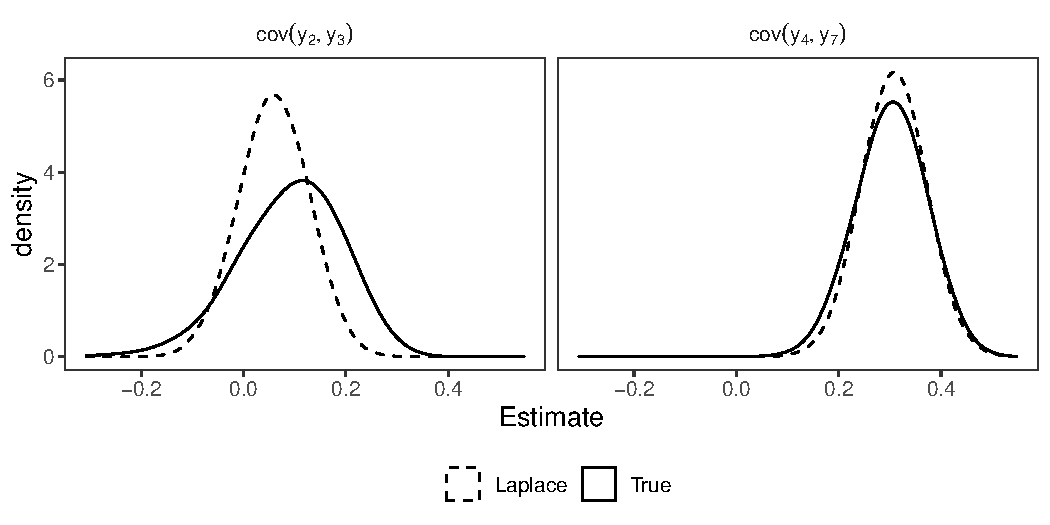
\includegraphics[width=0.9\textwidth]{fig/sampling_dist}
\caption{True and approximated sampling distributions for model residual covariances}
\label{fig:dist}
\end{figure}


\section{Discussion}

In this paper, we have outlined a new method for investigating local fit by approximating the probability that a parameter is meaningfully different than zero, which builds on the previous work of \textcite{Lee2016} and \textcite{Shi2019}.
By utilizing a Bayesian perspective, the resulting probability is arguably more intuitive to interpret.
The availability of a local fit assessment that does not require a complex interpretation may complement existing methods of model modification \citep[e.g., ][]{Sorbom1989, Kaplan1989, Wald1943}.
By using a straightforward approximation based on Laplace's method, many estimation complexities are avoided.
The approximation is also relatively fast compared to full Markov chain Monte Carlo methods.

Despite some potential advantages of the proposed method, there are also some important considerations.
The first consideration is determining the appropriate value of each parameter that should be used for computing the probability. 
For (standardized) factor loadings, we used a value of 0.30 suggested by \textcite{Benson1998} from EFA, but other values may be of interest.
Many of the decisions required for this method are likely to depend on the inferences of interest. 
For example, the threshold of meaningful correlation values will vary by application. 
Furthermore, researchers must decide the probability threshold needed in order to consider an omitted path meaningful. 
A fixed value for this probability may be counter productive because this probability is meant to be reflective of degree of evidence or belief about the magnitude of the parameter.
This view of probability is sometimes called the \textit{epistemic} or \textit{degree-of-belief} perspective of probability \citep[][, p. 14-15]{Levy2016, deFinetti1974}.

In conclusion, we have provided an approach to local fit assessment that provides researchers for an interpretable estimate of whether a modification will be of substantive importance.
The proposed approach allows for more information to be gained about the relationships in an observed dataset with respect to one's inferential interests.
This proposed approach is arguably intuitive and aligns with aims to search for sources of local (mis)fit rather than global fit.

% ============================= 
\newpage
\raggedright
%\bibliographystyle{apacite} 
% You may have to select another style. Remember: LaTeX, BibTeX, LaTeX, LaTex to get the citations to appear
%\raggedright
%\urlstyle{same}
%\bibliography{references}
\printbibliography
%~~
%%~~
\appendix

\section{Laplace Approximation Algorithm Steps} \label{app:algorithm}
Consider the model, Equation \ref{eq:cfa}, with corresponding full posterior in Equation \ref{eg:post}.
Laplace's method is utilized by constructing individual single parameter posteriors and sampling from each posterior separately.
This approach can be achieved through the following steps.
\begin{enumerate}
\item Fit the initially proposed CFA model ($M$) and save all the parameter estimates ($\theta$).
\item Construct a list of all possible parameters in $M$ that are not currently in the parameter space, such as all cross-loadings and error-covariances fixed to zero. Call these parameters $\theta^0$.
\item Fix the parameters in $M$ to those initially estimates, $\theta$. For each identified parameter in $\theta^0$, optimize the log posterior with respect $\theta^0$. This step with result in a posterior expected value for $\theta^0$ and the variance of this estimate.
\item Use the estimated expected value and variance as the parameters in a normal approximation to the posterior distribution. Sample $N$ times from this posterior and save these draws.
\item After all draws for each parameter are saved, standardized each draw based on the model estimated variances from $M$.
\item For each parameter, loop over all draws from the posterior to identify whether the sample exceeded the cutoff for the practical significance. Then, compute the mean of the 0/1 vector for each parameter. This mean is the posterior probability that the parameter is practically significant.
\end{enumerate}

\section{R Code for Laplace Approximation} \label{app:code}
\linespread{1}
\footnotesize
\singlespacing
\begin{lstlisting}
# ========================================== #
# ========================================== #
#   function: convert2matrix()
# ========================================== #
# use: takes vectors of positions in matrix
#       and values to create a possible 
#       sparse matrix
#
# arguments:
# theta - vector of parameters being optimized
# X     - obversed data
# model - list of model components (lambda...)
#
convert2matrix <- function(x, y, est) {
  Z<- matrix(NA, nrow=max(x), ncol=max(y))
  for(i in 1:length(est)){
    Z[x[i], y[i]] <- est[i]
  }
  Z
}

# ========================================== #
# ========================================== #
#   function: get_starting_values()
# ========================================== #
# use: obtain starting values, will work
#       for any parameters
#
# arguments:
# model - list of model components (lambda...)
#
get_starting_values <- function(model){
  lambdaMod <- model[[1]]
  phiMod <- model[[2]]
  psiMod <- model[[3]]
  
  # get length of each model element
  lam.num <- sum(is.na(c(lambdaMod))==T)
  phi.num <- sum(is.na(c(phiMod))==T)
  dphi.num <- sum(is.na(diag(phiMod))==T)
  odphi.num <- sum(is.na(phiMod[lower.tri(phiMod)])==T)
  psi.num <- sum(is.na(c(psiMod))==T)
  dpsi.num <- sum(is.na(diag(psiMod))==T)
  odpsi.num <- sum(is.na(psiMod[lower.tri(psiMod)])==T)
  # tau.num <- p
  # eta.num <- length(etaMod)
  
  k<-lam.num+phi.num+psi.num#+tau.num+eta.num
  sv<-numeric(k)
  # generate starting values
  sv.n1 <- sv.n2 <- sv.n3 <- sv.n4 <- sv.n5 <- NA
  if(lam.num==0){ 
    sv.n1 <- NA 
  }else{
    sv[1:(lam.num)] <- runif(lam.num, 0.6, 0.8)
    sv.n1 <-   paste0('lambda', 1:lam.num)
  }
  if(dphi.num==0){
    sv.n2 <- NA 
  }else{
    sv[(lam.num+1):(lam.num+dphi.num)]<- runif(dphi.num, 0.05, 1)
    sv.n2 <-   paste0('dphi', 1:dphi.num)
  }
  if(odphi.num==0){
    sv.n3 <- NA 
  }else{ 
    sv[(lam.num+dphi.num+1):(lam.num+phi.num)]<- runif(odphi.num, -.1, 0.1)
    sv.n3 <-  paste0('odphi', 1:odphi.num)
  }
  
  if(dpsi.num==0){
    sv.n4 <- NA 
  }else{ 
    sv[(lam.num+phi.num+1):(lam.num+phi.num+dpsi.num)] <- rep(0.2, dpsi.num)
    sv.n4 <-  paste0('dpsi', 1:dpsi.num)
  }
  
  if(odpsi.num==0){
    sv.n5 <- NA
  }else{ 
    sv[(lam.num+(phi.num + dpsi.num)+1):(lam.num+phi.num+psi.num)] <- runif(odpsi.num, -.05, 0.05)
    sv.n5 <-  paste0('odpsi', 1:odpsi.num)
  }
  #sv[(lam.num+phi.num+psi.num+1):(lam.num+phi.num+psi.num+tau.num)] <-sample(unlist(X), tau.num, replace=T)
  #sv[(lam.num+phi.num+psi.num+tau.num+1):(lam.num+phi.num+psi.num+tau.num+eta.num)] <-rnorm(eta.num, 0, 1)
  names(sv) <- na.omit(c(sv.n1, sv.n2, sv.n3, sv.n4, sv.n5)) #, paste0('tau', 1:tau.num), paste0('eta', 1:eta.num))
  return(sv)
}
# ========================================== #
# ========================================== #
#   function: trace()
# ========================================== #
# use: compute trace of matrix
#
trace <- function(A) {
  n <- dim(A)[1] # get dimension of matrix
  tr <- 0 # initialize trace value
  
  # Loop over the diagonal elements of the supplied matrix and add the element to tr
  for (k in 1:n) {
    l <- A[k,k]
    tr <- tr + l
  }
  return(tr[[1]])
}
# or one could do sum(diag(A))
# ========================================== #
# ========================================== #
#   function: XX2full()
# ========================================== #
# use: convert lower or upper matrix to full
up2full <- function(m) {
  m[lower.tri(m)] <- t(m)[lower.tri(m)]
  m
}
low2full <- function(m) {
  m[upper.tri(m)] <- t(m)[upper.tri(m)]
  m
}

# ========================================== #
# ========================================== #
#   function: progress_bar()
# ========================================== #
# use: makes the progress bar 
progress_bar <- txtProgressBar(min = 0, max = 2, style = 3)

# ========================================== #
# ========================================== #
#   function: get_prior_dens()
# ========================================== #
# use: gets the appropriate prior for the 
#       parameter of interest
#
get_prior_dens <- function(pvalue, pname,...){
  if(pname %like% 'lambda'){
    out <- dnorm(pvalue, 0, 1, log=T)
  }
  if(pname %like% 'dphi'){
    out <- dgamma(pvalue, 1, 0.5, log=T)
  }
  if(pname %like% 'odphi'){
    out <- dnorm(pvalue, 0, 1, log=T)
  }
  if(pname %like% 'dpsi'){
    out <- dgamma(pvalue, 1, 0.5, log=T)
  }
  if(pname %like% 'odpsi'){
    out <- dnorm(pvalue, 0, 1, log=T)
  }
  if(pname %like% 'eta'){
    out <- dnorm(pvalue, 0, 10, log=T)
  }
  if(pname %like% 'tau'){
    out <- dnorm(pvalue, 0, 32, log=T)
  }
  return(out)
}

# ========================================== #
# ========================================== #
#   function: get_log_post()
# ========================================== #
# use: uses the model, parameters, and data to
#       to calculate log posterior
#
# arguments:
# p        - names vector of parameters
# sample.data - data frame of raw data
# cfa.model - list of model components
#
get_log_post <- function(p, sample.data, cfa.model,...) {
  
  out <- use_cfa_model(p, cov(sample.data), cfa.model)
  
  log_lik <- sum(apply(sample.data, 1, dmvnorm,
                       mean=out[['tau']],
                       sigma=out[['Sigma']], log=T))
  
  log_prior<-0
  if(length(p)==1){
    log_prior <- get_prior_dens(p, names(p))
  } else {
    i <- 1
    for(i in 1:length(p)){
      log_prior <- log_prior + get_prior_dens(p[i], names(p)[i])
    }
  }
  log_post <- log_lik + log_prior
  log_post
}

# ========================================== #
# ========================================== #
#   function: use_cfa_model()
# ========================================== #
# use: take in parameters, data, and model to 
#         obtain the log-likelihood
#
# arguments:
# theta - vector of parameters being optimized
# sample.cov - samplecovariance matrix
# cfa.model - list of model parameters
use_cfa_model <- function(theta, sample.cov, cfa.model,...){
  # Compue sample statistics
  p<-ncol(sample.cov)
  S<-sample.cov
  
  # unpack model
  lambda <- cfa.model[[1]]
  phi <- cfa.model[[2]]
  psi <- cfa.model[[3]]
  #tau <- cfaModel[[4]]
  #eta <- cfaModel[[5]]
  
  # number factor loadings
  lam.num <- length(which(is.na(lambda)))
  lambda[which(is.na(lambda))] <- theta[1:lam.num]
  nF = ncol(lambda)
  # number elements in factor (co)variance matrix
  phi.num <- length(which(is.na(phi)))
  dphi.num <- sum(is.na(diag(phi))==T)
  odphi.num <- sum(is.na(phi[lower.tri(phi)])==T)
  if(phi.num > 0){
    if(dphi.num == 0){
      phi[which(is.na(phi))] <- theta[(lam.num+1):(lam.num+phi.num)]
    } else {
      diag(phi) <- theta[(lam.num+1):(lam.num+dphi.num)]
      phi[which(is.na(phi))] <- theta[(lam.num+dphi.num+1):(lam.num+phi.num)]
    }
  }
  phi <- low2full(phi) # map lower to upper
  
  # number elements in error (co)variance matrix
  psi.num <- length(which(is.na(psi)))
  dpsi.num <- sum(is.na(diag(psi))==T)
  odpsi.num <- sum(is.na(psi[lower.tri(psi)])==T)
  if(psi.num > 0){
    if(dpsi.num == 0){
      psi[which(is.na(psi))] <- theta[(lam.num+1):(lam.num+psi.num)]
    } else {
      diag(psi) <- theta[(lam.num+1):(lam.num+dpsi.num)]
      psi[which(is.na(psi))] <- theta[(lam.num+dpsi.num+1):(lam.num+psi.num)]
    }
  }
  psi <- low2full(psi)
  # number of factor scores
  #eta.num <- length(eta)
  #eta <- matrix(theta[(lam.num+phi.num+psi.num+tau.num+1):(lam.num+phi.num+psi.num+tau.num+eta.num)],
  #              nrow=nF)
  # mean center eta
  #for(i in 1:nF){
  #  eta[i, ] <- eta[i,] - mean(eta[,i])
  #}
  
  # # number of intercepts
  # tau.num <- length(tau)
  # tau <- matrix(theta[(lam.num+phi.num+psi.num+1):(lam.num+phi.num+psi.num+tau.num)], ncol=1)
  # tau <- repeat_col(tau, ncol(eta))
  
  # compute model observed outcomes
  #Y <- tau + lambda%*%eta
  tau <- numeric(p)
  # compute model implied (co)variance matrix
  Sigma<-lambda%*%phi%*%(t(lambda)) + psi
  
  #return fit value 
  out <- list(Sigma, lambda, phi, psi, tau)
  names(out) <- c('Sigma', 'lambda', 'phi', 'psi', 'tau')
  return(out)
}



# ========================================== #
# ========================================== #
#   function: laplace_local_fit()
# ========================================== #
# use: uses the fittes lavaan object to run
#       the proposed method
#
# arguments:
# fit       - fitted lavaan model
# standardized - logical for whether to standardize
# cut.load  - cutoff for value of loading to care about default = 0.3 
# cut.cov   - cutoff for value of covariances to care about default = 0.1
# opt       - list of parameters to pass to interior functions
# sum.print - logical indicator of whether to print the summary table upon completion
# counter   - logical indicator of whether to print out a (.) after each
#               parameter is completed
#
laplace_local_fit <- function(fit, cut.load = 0.3, cut.cov = 0.1, standardize=T,
                              opt=list(scale.cov=1, no.samples=1000),
                              all.parameters=F,
                              sum.print=F, pb=T,...){
  
  # Observed Data
  sampleData <- fit@Data@X[[1]]
  # sample covariance matrix
  sampleCov <- fit@SampleStats@cov[[1]]
  
  # extract model
  extractedLavaan <- lavMatrixRepresentation(partable(fit))
  
  factNames <- unique(extractedLavaan[extractedLavaan[,"mat"]=="lambda", "lhs"])
  varNames <- unique(extractedLavaan[extractedLavaan[,"mat"]=="lambda", "rhs"])
  # extract factor loading matrix
  lambda <- extractedLavaan[ extractedLavaan$mat == "lambda" ,]
  lambda <- convert2matrix(lambda$row, lambda$col, lambda$est)
  colnames(lambda) <- factNames
  rownames(lambda) <- varNames
  # extract factor covariance matrix
  phi <- extractedLavaan[ extractedLavaan$mat == "psi" ,]
  phi <- convert2matrix(phi[,'row'], phi[,'col'], phi[,'est'])
  phi <- up2full(phi)
  colnames(phi) <- rownames(phi) <- factNames
  # extract error covariance matrix
  psi <- extractedLavaan[ extractedLavaan$mat == "theta" ,]
  psi <- convert2matrix(psi[,'row'], psi[,'col'], psi[,'est'])
  psi[upper.tri(psi)] <- 0
  colnames(psi) <- rownames(psi) <- varNames
  
  
  # need to create list of all NA parameters in the above matrices
  
  if(all.parameters == T){
    lambdaA <- lambda
    phiA <- phi
    psiA <- psi
    
    lambdaA[!is.na(lambdaA)] <- NA
    phiA[!is.na(phiA)] <- NA
    psiA[!is.na(psiA)] <- NA
    
  } else{
    lambdaA <- lambda
    phiA <- phi
    psiA <- psi
    
  }
  
  lamList <- as.matrix(which(is.na(lambdaA), arr.ind = T))
  il <- nrow(lamList)
  phiList <- as.matrix(which(is.na(phiA), arr.ind = T))
  ip <- il + nrow(phiList)
  psiList <- as.matrix(which(is.na(psiA), arr.ind = T))
  it <- ip + nrow(psiList)
  modList <- rbind(lamList, phiList, psiList)
  # number of variables
  # create names for each condition
  vnlamList <- lamList
  vnlamList[,2] <- paste0(factor(vnlamList[,2], levels = order(unique(vnlamList[,2])),labels=factNames))
  vnlamList[,1] <- rownames(lamList)
  vnlamList[,2] <- paste0(vnlamList[,2],"=~",vnlamList[,1])
  vnphiList <- phiList
  if(nrow(phiList)>0){
    vnphiList[,1] <- paste0(factor(phiList[,1], levels = order(unique(vnphiList[,1])),labels=factNames))
    vnphiList[,2] <- paste0(factor(phiList[,2], levels = order(unique(phiList[,2])),labels=factNames))
  }
  vnpsiList <- psiList
  vnpsiList[,1] <- rownames(psiList)
  vnpsiList[,2] <- paste0(vnpsiList[,1],"~~y", psiList[,2])
  nameList <- rbind(vnlamList, vnphiList, vnpsiList)
  # ========================================================== #
  # ========================================================== #
  # iterate around this function
  fitResults <- matrix(nrow=opt[[2]], ncol=it)
  # progress bar
  if(pb==T) progress_bar <- txtProgressBar(min = 0, max = it, style = 3)
  iter <- 1
  for(iter in 1:it){
    
    # extract iteration information from modList
    x <- modList[iter, ]
    
    # do we need to update lambda?
    if(iter <= il){
      Q <- lambda
      Q[is.na(Q)] <- 0
      Q[x[1], x[2]] <- NA
      lambdaMod <- Q
    } else {
      Q <- lambda
      Q[is.na(Q)] <- 0
      lambdaMod <- Q
    }
    
    # update phi?
    if(iter > il & iter <= ip){
      Q <- phi
      Q[is.na(Q)] <- 0
      Q[x[1], x[2]] <- NA
      phiMod <- Q
    } else {
      Q <- phi
      Q[is.na(Q)] <- 0
      phiMod <- Q
    }
    
    # update psi?
    if(iter > ip){
      Q <- psi
      Q[is.na(Q)] <- 0
      Q[x[1], x[2]] <- NA
      psiMod <- Q
    } else {
      Q <- psi
      Q[is.na(Q)] <- 0
      psiMod <- Q
    }
    
    # combine into a single list
    cfaModel <- list(lambdaMod, phiMod, psiMod) #, tauMod, etaMod
    
    #print(cfaModel)
    # get starting values
    inits <- get_starting_values(cfaModel) 
    
    # use optim() to run simulation
    fit <- optim(inits, get_log_post, control = list(fnscale = -1),
                 hessian = TRUE,
                 sample.data=sampleData, cfa.model=cfaModel)
    param_mean <- fit$par # numerical deriv
    # compute hess at param_mean
    #hess <- numDeriv::hessian(model, param_mean, ...)
    #param_cov_mat <- solve(-hess)
    param_cov_mat <- solve(-fit$hessian)
    
    # scaled covariance matrix (artifically inflate uncertainty)
    scale.cov = opt[[1]]
    A <- diag(scale.cov, nrow=nrow(param_cov_mat), ncol=ncol(param_cov_mat))
    param_cov_mat <- A%*%param_cov_mat%*%t(A)
    
    # sample
    no.samples=opt[[2]]
    fitResults[,iter] <- mcmc(rmvnorm(no.samples, param_mean, param_cov_mat))
    
    if(pb == T) setTxtProgressBar(progress_bar, iter)
  }
  # ========================================================== #
  # ========================================================== #
  
  colnames(fitResults) <- nameList[,2, drop=T]
  
  # Next, standardized (if desired) default
  if(standardize==T){
    # standardize
    obs.var <- extractedLavaan[extractedLavaan[,"mat"]=="theta", ]
    obs.var <- obs.var[which(obs.var$lhs == obs.var$rhs), c("lhs", "est")]
    
    fct.var <- extractedLavaan[extractedLavaan[,"mat"]=="psi", ]
    fct.var <- fct.var[which(fct.var$lhs == fct.var$rhs), c("lhs", "est")]
    
    all.var <- rbind(obs.var, fct.var)
    
    fitResults <- fitResults
    p <- colnames(fitResults)
    i <- 1
    for(i in 1:length(p)){
      unstd <- fitResults[,i]
      
      if(p[i] %like% "=~"){
        pp <- strsplit(p[i], "=~") %>% unlist()
        sigjj <- sqrt(all.var[all.var[,1] == pp[1], 2])
        sigii <- sqrt(all.var[all.var[,1] == pp[2], 2])
        std <- unstd*sqrt(sigjj/sigii) # bollen (1989, p. 349)
      }
      
      if(p[i] %like% "~~"){
        pp <- strsplit(p[i], "~~") %>% unlist()
        sigjj <- sqrt(all.var[all.var[,1] == pp[1], 2])
        sigii <- sqrt(all.var[all.var[,1] == pp[2], 2])
        std <- unstd/(sigjj * sigii) # bollen (1989, p. 349)
      }
      
      fitResults[,i] <- std
    }
  }
  # now, compute and format summary statistics
  sumResults <- data.frame(matrix(nrow=ncol(fitResults), ncol=9))
  colnames(sumResults) <- c("Parameter","Prob", "mean", "sd", "p0.025", "p0.25", "p0.5", "p0.75", "p0.975")
  sumResults[,1] <- colnames(fitResults)
  
  sumResults[,3:9] <- t(apply(fitResults, 2, function(x){
    c(mean(x, na.rm=T), sd(x, na.rm=T),
      quantile(x, c(0.025, 0.25, 0.5, 0.75, 0.975), na.rm=T))
  }))
  
  # compute probability of meaningfulness
  # depends on parameter
  # cut.load = 0.3
  # cut.cov = 0.1
  p <- colnames(fitResults)
  for(i in 1:ncol(fitResults)){
    x <- fitResults[,i, drop=T]
    if(p[i] %like% "=~"){
      pv <- mean(ifelse(abs(x) >= cut.load, 1, 0))
    }
    if(p[i] %like% "~~"){
      pv <- mean(ifelse(abs(x) >= cut.cov, 1, 0))
    }
    sumResults[i, 2] <- pv
  }
  sumResults <- arrange(sumResults, desc(Prob))
  colnames(sumResults) <- c("Parameter","Pr(|theta|>cutoff)", "mean", "sd", "p0.025", "p0.25", "p0.5", "p0.75", "p0.975")
  sumResults[,2:9] <- round(sumResults[,2:9], 3)
  cat("\n")
  if(sum.print==T) print(sumResults, row.names = FALSE)
  
  # convert to data.frame
  fitResults <- as.data.frame(fitResults)
  out <- list(fitResults, sumResults)
  names(out) <- c("All Results", "Summary")
  
  return(out)
}
\end{lstlisting}


\end{document}
